Verze 1.6.7 umožňovala zahrnutí rovnovážné sorpce a duální porozity v modelu 
explicitního transportu. Ve verzi 1.7.0 byla tato funkcionalita zachována, ale 
parametry obou modelů byly zadávány pomocí tříd pro časo-prostorová pole což 
vedlo k dramatickému zpomalení. Byly implementovány třídy pro výpočet rozpadů a 
jednoduchých reakcí, ale pouze v kapalné fázi, tj. bez uvažování sorpce či 
duální porozity. Sorpce, duální porozita i jednoduché reakce byly implementovány 
pouze na explicitní transport pomocí metody štěpení operátoru. 

Ve verzi 1.8.0 je také použita metoda štěpení operátoru, ale je možné kombinovat 
jednotlivé lokální modely. V jednom časovém kroku se nejprve spočítá transport 
látky bez dalších vlivů a následně jsou v každém elementu spočteny
modely reakčního členu: nerovnovážná výměna s duálními póry, rozpady a 
jednoduché reakce v primárních i duálních pórech v rozpuštěné i sorbované fázi a 
nakonec je spočtena rovnovážná sorpce v primárních i duálních pórech. Tyto 
modely je možno kombinovat jak je znázorněno na Obrázku 
\ref{fig:reaction_term}. Uživatel tak může volit jak komplexní děje chce 
reakčním členem popsat. Může to být pouhá reakce typu "Jaderný rozpad" nebo 
komplexní schéma zahrnující duální porozitu, jiný druh sorpce pro mobilní a 
imobilní póry a čtyři druhy reakcí v roztoku/hornině v mobilních/imobilních 
pórech.

\begin{figure}[h]
 \centering
 \includegraphics[scale=0.4]{./reaction_term.pdf}
 % reaction_term.pdf: 842x595 pixel, 72dpi, 29.70x20.99 cm, bb=0 0 842 595
 \caption{Struktura reakčního členu. Dělený box má v horní části fyzikální 
kontext a v dolní části výčet modelů, které lze v daném kontextu použít.}
 \label{fig:reaction_term}
\end{figure}


Technicky umožňujeme použití 
metody štěpení operátoru pro explicitní i implicitní transport, nicméně v 
případě implicitního transportu je třeba volit dostatečně krátký časový krok.

\subsubsection{Duální porozita}
Model umožňuje popsat retenční vlastnosti slepých pórů a puklin, které se 
efektivně projevují při simulacích na velkém měřítku. Porézní médium je 
rozděleno na mobilní póry, mobilní porozita $\theta_m$, a imobilní póry, 
imobilní porozita $\theta_i$. Mezi těmito póry nedochází k proudění vody, ale 
dochází k výměně látky difúzí. Tato nerovnovážná výměna je řízena jednoduchou 
lineární soustavou obyčejných diferenciálních rovnic:
\begin{align}
    \vartheta_m \partial_t c_m &= D_{dp} ( c_i - c_m), 
\label{eqn:dual_porosity_ode1}\\
    \vartheta_i \partial_t c_i &= D_{dp} ( c_m - c_i), 
\label{eqn:dual_porosity_ode2}
\end{align}
kde $c_m$ je koncentrace látky v mobilní zóně, $c_i$ je koncentrace látky v 
imobilní zóně a $D_{dp}$ je koeficient difúze mezi zónami.


\subsubsection{Sorpce}
Implementace rovnovážných sorpcí byla kompletně předělána. Byla zachována 
možnost zadávat všechny parametry pomocí časo-prostorových polí, nicméně pro 
případ parametrů konstantních na jednotlivých regionech je implementován výpočet 
pomocí předpočítaných interpolací, který umožňuje efektivní výpočet jak pro 
lineární tak nelineární sorpční izotermy. Výpočet rovnovážné sorpce pro jednu 
látku spočívá v řešení soustavy rovnic sestávající z bilance hmoty,
\begin{equation}
\label{eq:mass_balance_sorption}
\th \varrho_l c_l + (1-\th) \varrho_s M_s c_s = c_T = const.
\end{equation}
a z empirického vztahu nazývaného sorpční izoterma:
\[
    c_s=f(c_l).
\]
V těchto rovnicích jsou neznámé hmotnostní koncentrace látky v roztoku $c_l$ a 
molární koncentrace látky v hornině $c_s$, další veličiny jsou hustota 
rozpouštědla (vody) $\varrho_l$, hustota horniny $\varrho_s$, molární hmotnost 
látky $M_s$ a celková koncentrace $c_T$. Výpočet probíhá tak, že po transportu 
látky je porušena sorpční rovnováha, z rovnice \eqref{eq:mass_balance_sorption} 
se vypočte celková koncentrace (celková hustota hmotnosti látky) a pak se 
naleznou nové rovnovážné hodnoty $c_s$, $c_l$.

Momentálně jsou implementovány lineární, Langmuierova a Freundlichova izoterma. 
Obvykle jsou parametry rovnice závislé pouze na látce a regionu a pro 
jednotlivé elementy jednoho regionu je třeba spočítat rovnovážné koncentrace pro 
různé hodnoty celkové koncentrace $c_T$. V tom případě uvažujeme graf izotermy 
v otočené soustavě (viz. Obr. 3).

Hodnoty veličiny
\[
    Y=-\mu_s c_l + \mu_l c_s =  -M_s(1-\theta) \varrho_s c_l + \theta\rho_l 
\]

v závislosti na $c_T$ jsou tabelovány a mezihodnoty dopočítávány lineární 
interpolací. Rovnovážné koncentrace pak dostaneme zpětným otočením:
\[
    c_l = \frac{\mu_l c_T + \mu_s Y}{\mu_s^2+\mu_l^2},\quad c_s = 
\frac{-\mu_s c_T - \mu_l Y}{\mu_s^2 + \mu_l^2}.
\]

Tímto způsobem jsme schopni počítat i nelineární sorpce stejně efektivně jako 
lineární. Tabulka \ref{tab:isoterm_timing} shrnuje výsledky benchmarkových 
testů. Porovnáváme čas výpočtu sorpcí (v sekundách) pro tři různé izotermy a 
tři 
různé verze kódu. V prvním sloupci jsou časy původní implementace z verze 1.6.7. 
Ve druhém sloupci jsou výsledky pro implementaci využívající interpolace při 
prostorově konstantních parametrech izoterm. Dosáhli jsme značného zrychlení 
pro 
nelineární izotermy. Ve třetím sloupečku jsou časy při použití  plně prostorově 
závislých parametrů, kde je nelineární rovnice řešena pro každý element, látku 
a časový krok. Zde je ještě prostor pro optimalizace. Přibližně $11$s trvá 
výpočet prostorově závislých parametrů nicméně i po odečtení tohoto konstantního 
faktoru jsou časy výrazně horší než pro verzi 1.6.7. Tuto variantu však 
neplánujeme používat pro rozsáhlé oblasti a hoší výkon proto nepředstavuje 
praktické omezení. Další optimalizace by bylo možné dosáhnout použitím Newtonovy 
metody pro řešení nelineárních rovnic, jako tomu bylo ve verzi 1.6.7. Zde 
používáme metodu pomalejší, ale stabilnější a umožňující snadné přidávání nových 
izoterm.

\renewcommand{\arraystretch}{1.5}
\begin{table}
\begin{center}
\begin{tabular}{|l||c|c|c|}
\hline
izoterma & verze 1.6.7 & v. 1.8.0 (interpolace) & v. 1.8.0 (přímý výpočet) \\
\hline
Lineární & 1.58        & 1.48                   & 28\\
Langmuirova & 5.87     & 1.44                   & 36\\
Freundlichova& 19.21   & 1.50                   & 44\\
\hline
\end{tabular}
\end{center}
\caption{\label{tab:isoterm_timing}
Doba výpočtu sorpcí v sekundách pro různé izotermy a tři různé verze 
kódu: původní, s použitím interpolací a při plně prostorově závislých 
parametrech.}
\end{table}
